\chapter{Introdução}
O crescimento no consumo de energia cada vez mais vem aumentando conforme os anos. No
ano de 2014 o Brasil consumiu 531.1 TWh, resultando em um aumento de 2.9\% comparado à 2013 \cite{balanco_energetico}.

O Brasil possui uma matriz energética predominantemente renovável tendo como ênfase a geração hidráulica. As fontes renováveis correspondem à 84.1\% e não renováveis 26.9\%, conforme ilustrado na imagem \ref{consumo-2014}.

\begin{figure}[h]
    \centering
    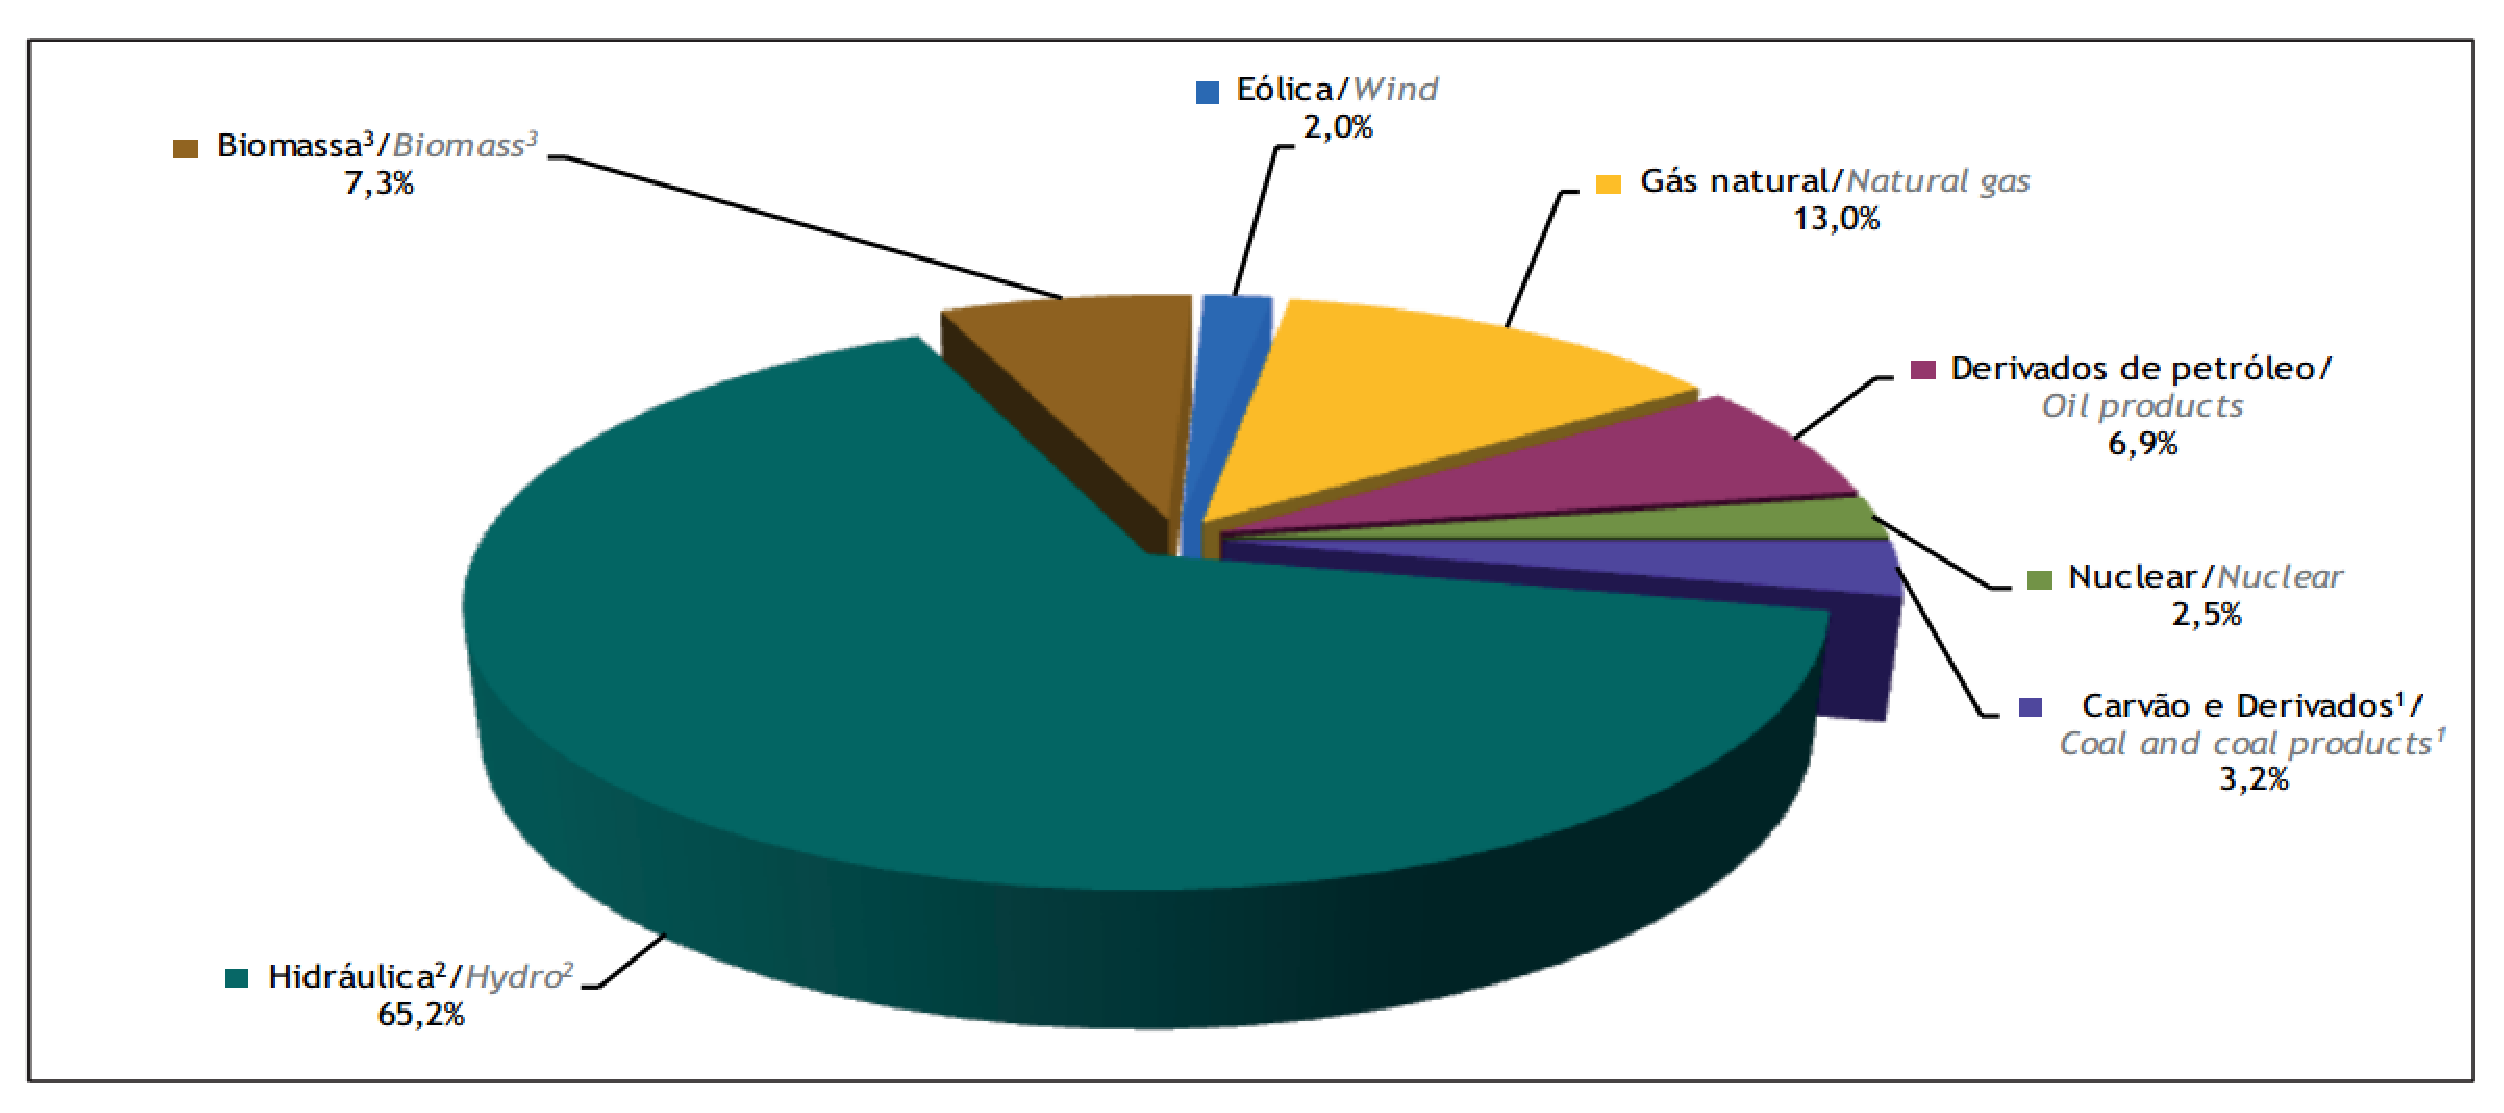
\includegraphics[keepaspectratio=true,scale=0.4]{figuras/consumo_energia_2014.eps}
    \caption{Oferta Interna de Eletricidade no Brasil em 2014. Fonte: \cite{balanco_energetico}}
    \label{consumo-2014}
\end{figure}

Uma pequena parte do consumo total de energia elétrica do Brasil é realizada por prédios públicos, sendo
esses responsáveis pela prestação de serviços à população. Em 2014, o total de energia elétrica consumida
pelos mesmos foi de 12.61 TWh, representando 2.4\% do total consumido pelo país \cite{balanco_energetico}.

No ano de 2015 foi realizado um reajuste tarifário da energia elétrica correspondente à 33\% para clientes residenciais e 32,5\% para empresas, indústrias e comércios \cite{aumento_energia}, gerando altos gastos.

Dentre as alternativas para reduzir o consumo de energia elétrica encontram-se o uso de equipamentos mais eficientes, certificações Procel\footnote{\url{www.procelinfo.com.br/selo_procel_edificacoes/}}, uso racional da energia e afins, porém, quando se trata de instalações de grande porte, como Universidades e órgãos públicos em geral, percebe-se que um dos grandes problemas enfrentado é a falta de monitoramento adequado do uso de energia elétrica.

\#TODO software gerando eficiencia na gestão publica + sustentabilidade.

\section{Contexto}
Em Maio de 2016, a Prefeitura de Campus da Universidade de Brasília (UnB) aprovou um projeto de gerenciamento energético da própria Universidade, objetivando que cada Campus da instituição (Asa Norte, Ceilândia, Gama e Planaltina) seja responsável por realizar, com o auxílio de transdutores, seu próprio monitoramento de energia e enviar essas informações coletadas para o Campus Darcy Ribeiro, o qual funcionaria como uma Central. As etapas do projeto foram dividas em:
\begin{itemize}
    \item Determinação de pontos críticos para monitoramento;
    \item Instalação de transdutores nos pontos críticos;
    \item Desenvolvimento de um sistema \textit{web} capaz de comunicar-se com os transdutores e tratar os dados de energia.
\end{itemize}

Num primeiro momento foi selecionado o Campus do Gama (FGA)\footnote{\url{https://fga.unb.br/}} para que
fossem realizadas as instalações de transdutores. Tal escolha foi definida pela complexidade das instalações, visto que o Campus possui apenas 8 anos de funcionamento, uma menor proporção comparado ao Campus Darcy Ribeiro e pelo fato da equipe responsável pela execução do projeto, tabela \ref{equipe_projeto}, encontrar-se estabelecida no mesmo.

\begin{table}[!htbp]
    \centering
    \caption{Equipe Execução Projeto. Fonte: autor}
    \label{equipe_projeto}
    \begin{tabular}{|p{5cm}|p{2cm}|p{3cm}|}
    \hline
    \textbf{Membro}                                                                    & \textbf{Titulação} & \textbf{Função}        \\\hline
    Brenddon Gontijo Furtado                                                  & Estudante & Desenvolvedor \\\hline
    Loana Nunes Valesco                                                       & Doutor    & Coordenador   \\\hline
    Alex Reis                                                                 & Doutor    & Pesquisador   \\\hline
    Roberto Miranda Meirelles                                                 & Doutor    & Pesquisador   \\\hline
    \end{tabular}
\end{table}

Após realizada a instalação dos transdutores restava apenas o desenvolvimento do sistema, para isso realizaram-se reuniões com a Dra. Loana Nunes Velasco, das quais foram definidos o nome do sistema, SME-UnB (Sistema de Monitoramento Energético - Universidade de Brasília), e suas principais funcionalidades:
\begin{itemize}
    \item Geração de relatórios
    \item Gráficos de consumo, demanda e afins
    \item Monitoramento temporal de transdutores
    \item Simulação de fatura
    \item Sistema de alarme para eventos indesejados
\end{itemize}

Para o contexto deste trabalho definiu-se a realização de uma parte das funcionalidades do SME-UnB.

\section{Objetivo Geral}
Desenvolver sistema web capaz de monitorar, em tempo real, medições de energia coletadas por transdutores
instalados em quadros de energia da Universidade de Brasília.

\subsection{Objetivos Específicos}
O sistema deve ser capaz de:
\begin{itemize}
    \item Cadastrar/Editar/Remover transdutores.
    \item Utilizar rede da Universidade para comunicar-se com transdutores.
    \item Realizar a coleta de dados de forma automatizada e temporizada.
    \item Mostrar aos usuários os dados de energia coletados.
\end{itemize}

\section{Metodologia Utilizada}
A metodologia abordada neste trabalho teve como base o desenvolvimento de um \textit{software} livre \footnote{\url{http://www.gnu.org/philosophy/free-sw.pt-br.html}} utilizando-se dos princípios empíricos de desenvolvimento ágil \footnote{\url{http://agilemanifesto.org/}} de \textit{software} juntamente com práticas do Scrum \footnote{\url{http://www.scrumguides.org/}} e \textit{Extreme Programming} \footnote{\url{http://www.extremeprogramming.org/}}.

\section{Estruturação do Trabalho}
O trabalho encontra-se estruturado da seguinte maneira:

\begin{itemize}
    \item Capítulo 2: abordará os métodos empíricos em engenharia de \textit{software} utilizados para
    auxiliar no desenvolvimento do sistema.
    \item Capítulo 3: abordará como estruturou-se a gerência de configuração.
    \item Capítulo 4: abordará as princípais tecnologias \textit{web} e protocolos de comunicação utilizados.
    \item Capítulo 5: abordará a evolução do desenvolvimento do sistema, relatando o que foi realizado durante cada \textit{sprint}.
    \item Capitulo 6: abordará uma conclusão preliminar sobre o que foi/resta a ser desenvolvido.
\end{itemize}